\documentclass[../relazione.tex]{subfiles}

\begin{document}
\section{Accessibilità}
	\subsection{Chiarezza e semplicità}
		È stato scelto un font molto chiaro per permettere all'utente di leggere senza sforzi il contenuto. Si è cercato di mantenere la semplicità in ogni parte del sito, sia nel contenuto che nella presentazione.\\
		Per maggiore chiarezza, ma anche per permettere all'utente di salvare una pagina del sito tra i preferiti senza che ciò crei confusione, il tag \texttt{title} nell'\texttt{head} di ogni pagina è stato definito dal particolare al generale.
			
	\subsection{Il colore}
		Le disabilità visive testate sul sito sono le seguenti: deuteranopia, monochromacy, partialMonochromacy, protanopia e tritanopia.\\
		L'esito è stato che indipendentemente dal tipo di malattia il sito si presenta in maniera chiara e accessibile.\\\\
		Una nota particolare va fatta per i \texttt{link}: essi sono colorati di rosa salmone, però sono rafforzati dal grassetto proprio per renderli maggiormente distinguibili anche nel caso in cui l'utente non sia in grado di vedere il colore; a tal riguardo, il caso più lampante per il nostro sito è la monochromacy: se non fossero in grassetto i link sarebbero difficilmente distinguibili dal resto del testo.\\\\
		Di seguito sono riportati una serie di esempi di una pagina del sito vista da una persona con disabilità visiva.
	\begin{figure}[H]
	\centering
		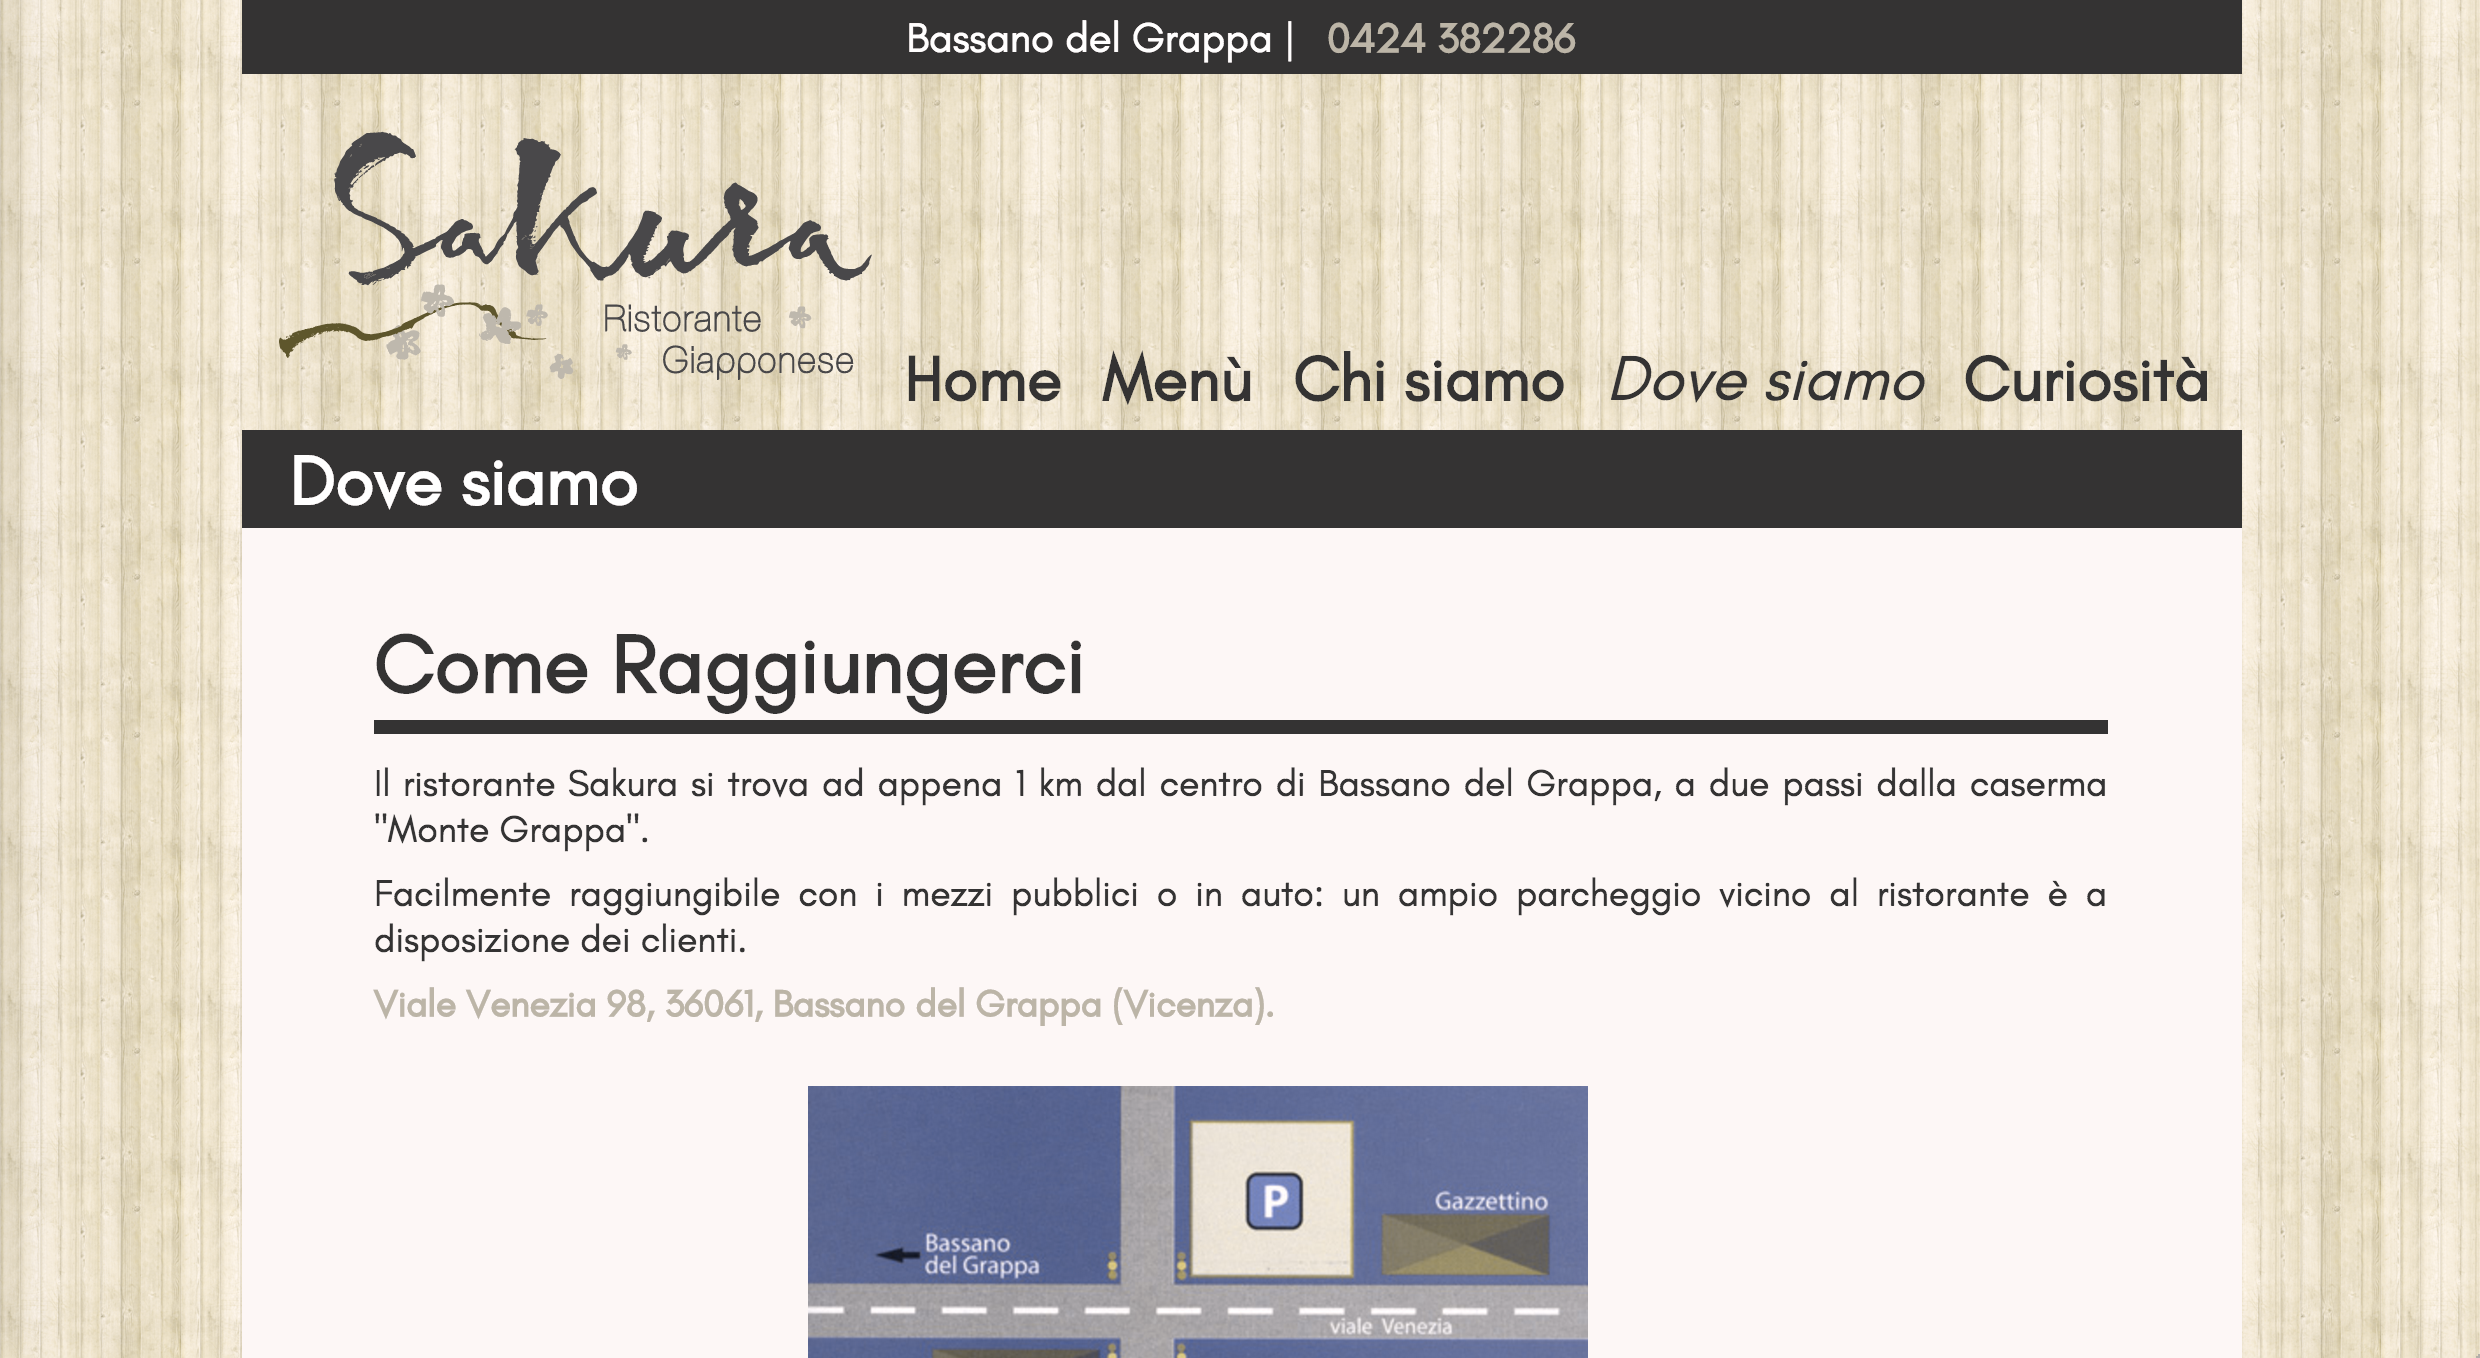
\includegraphics[width=\textwidth]{images/colorblindness/protanopia}
		\caption{Esempio di pagina vista da chi soffre di protanopia}
		\label{fig:Esempio di pagina vista da chi soffre di protanopia}
	\end{figure}
	\begin{figure}[H]
	\centering
		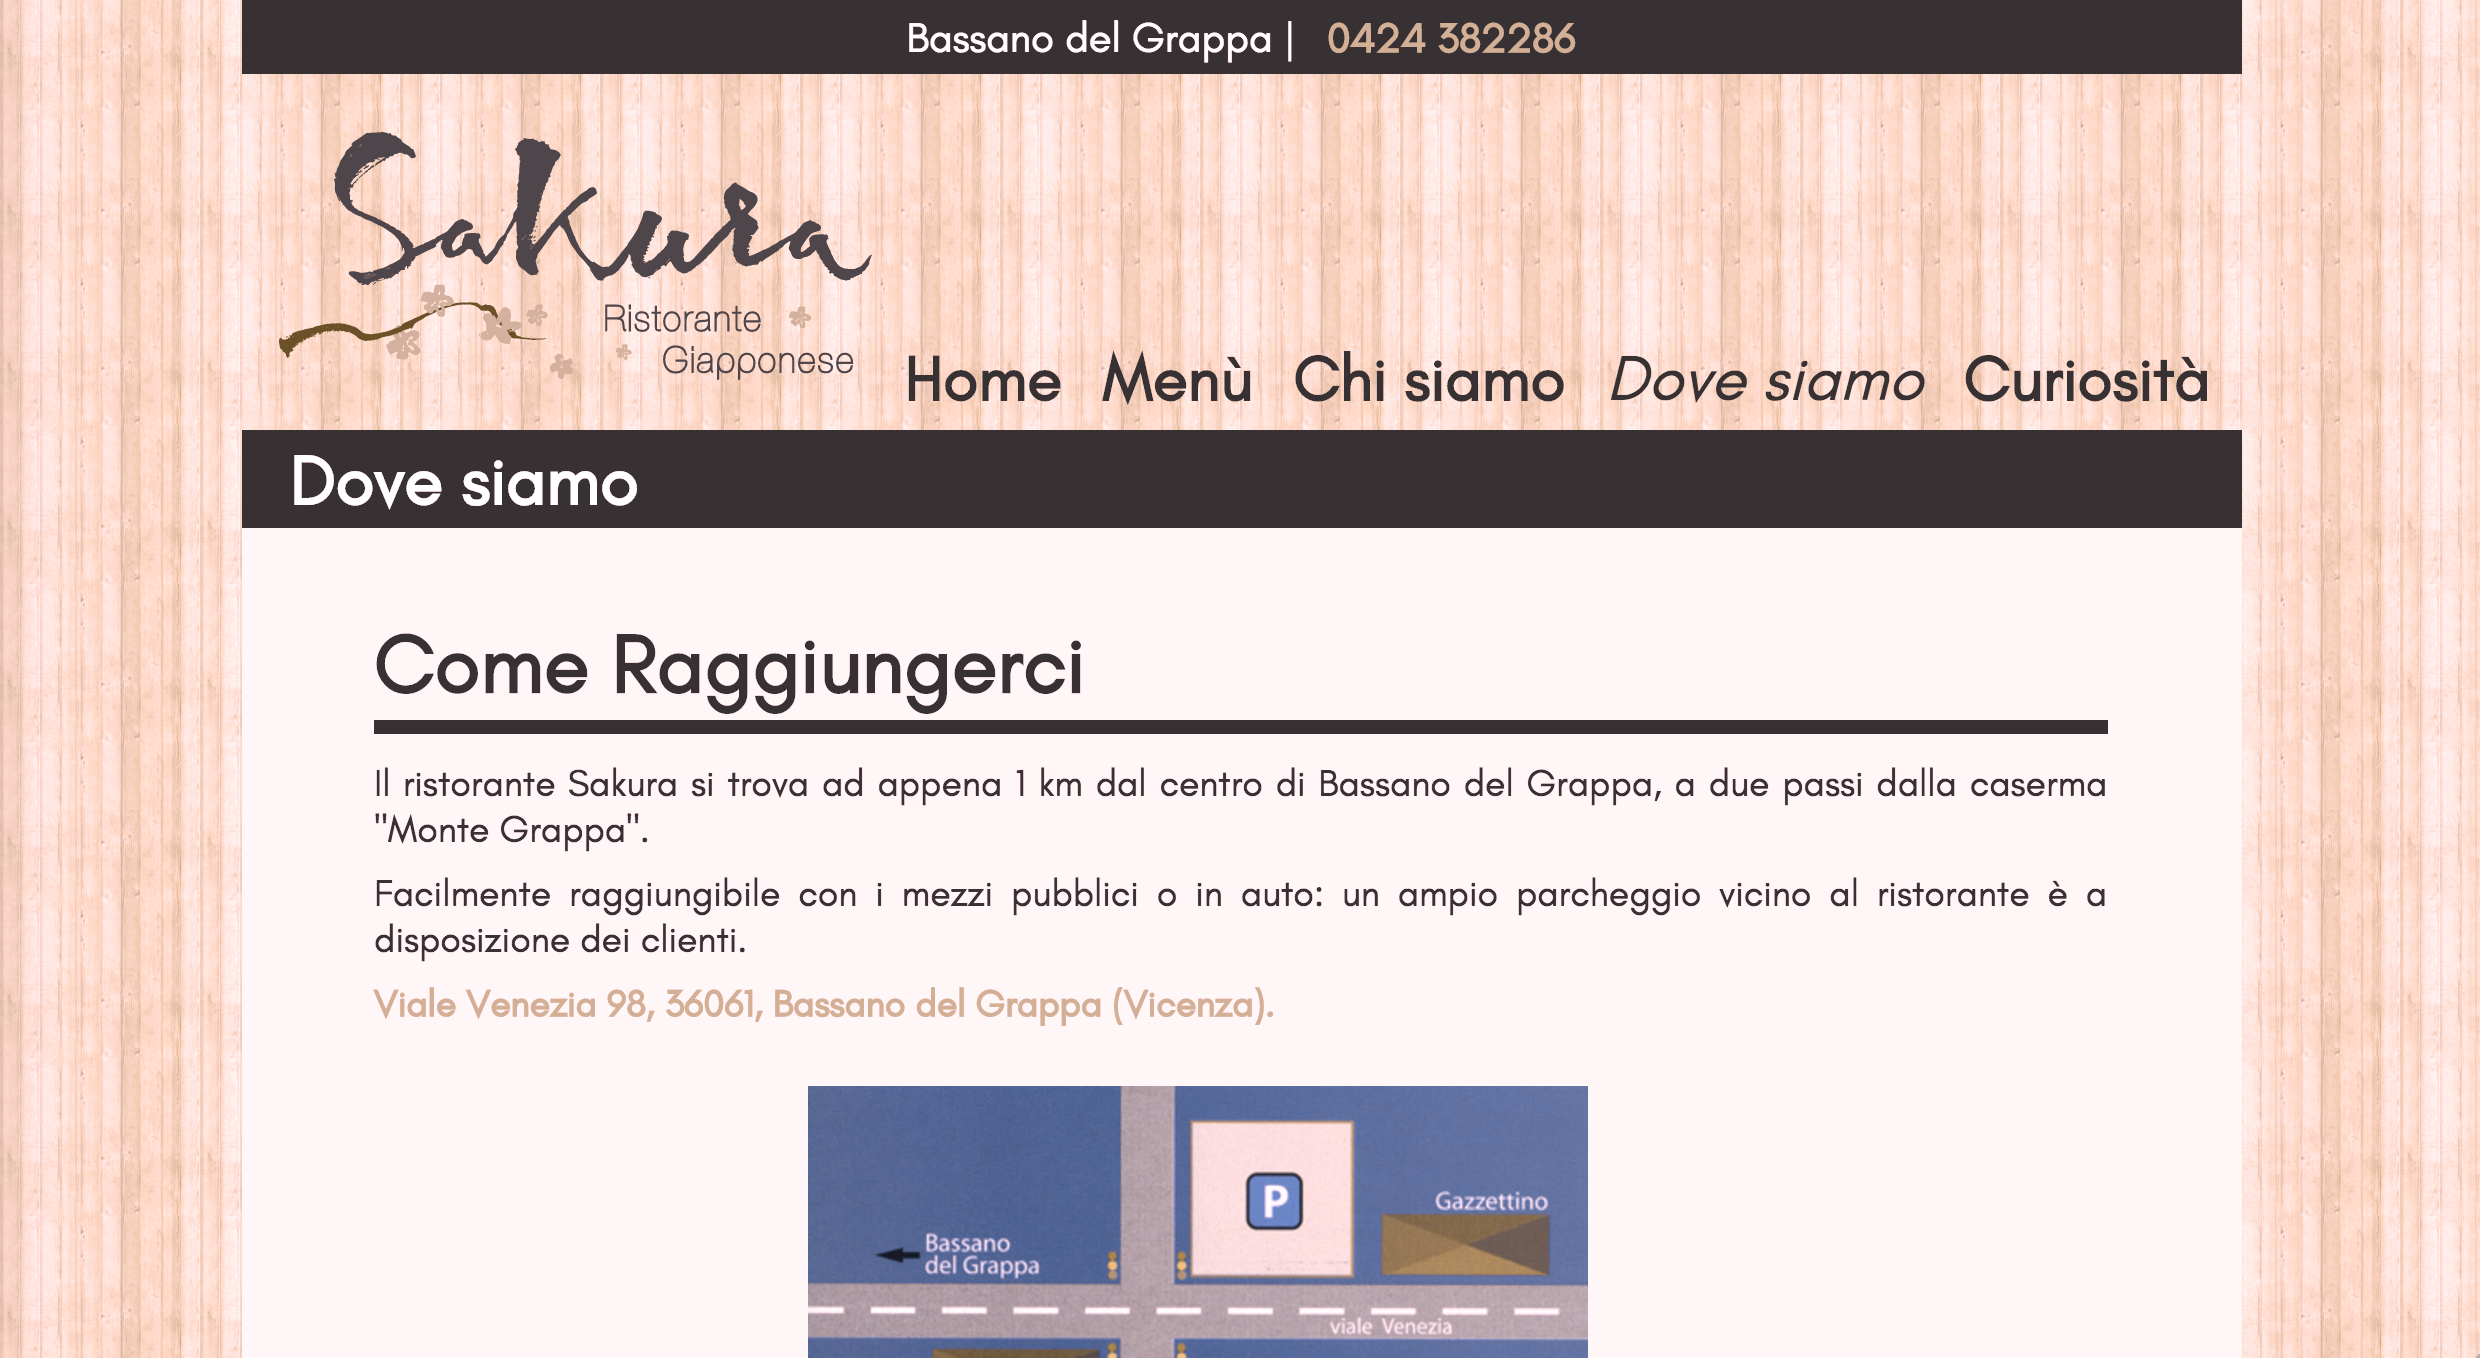
\includegraphics[width=\textwidth]{images/colorblindness/deuteranopia}
		\caption{Esempio di pagina vista da chi soffre di deuteranopia}
		\label{fig:Esempio di pagina vista da chi soffre di deuteranopia}
	\end{figure}
	\begin{figure}[H]
	\centering
		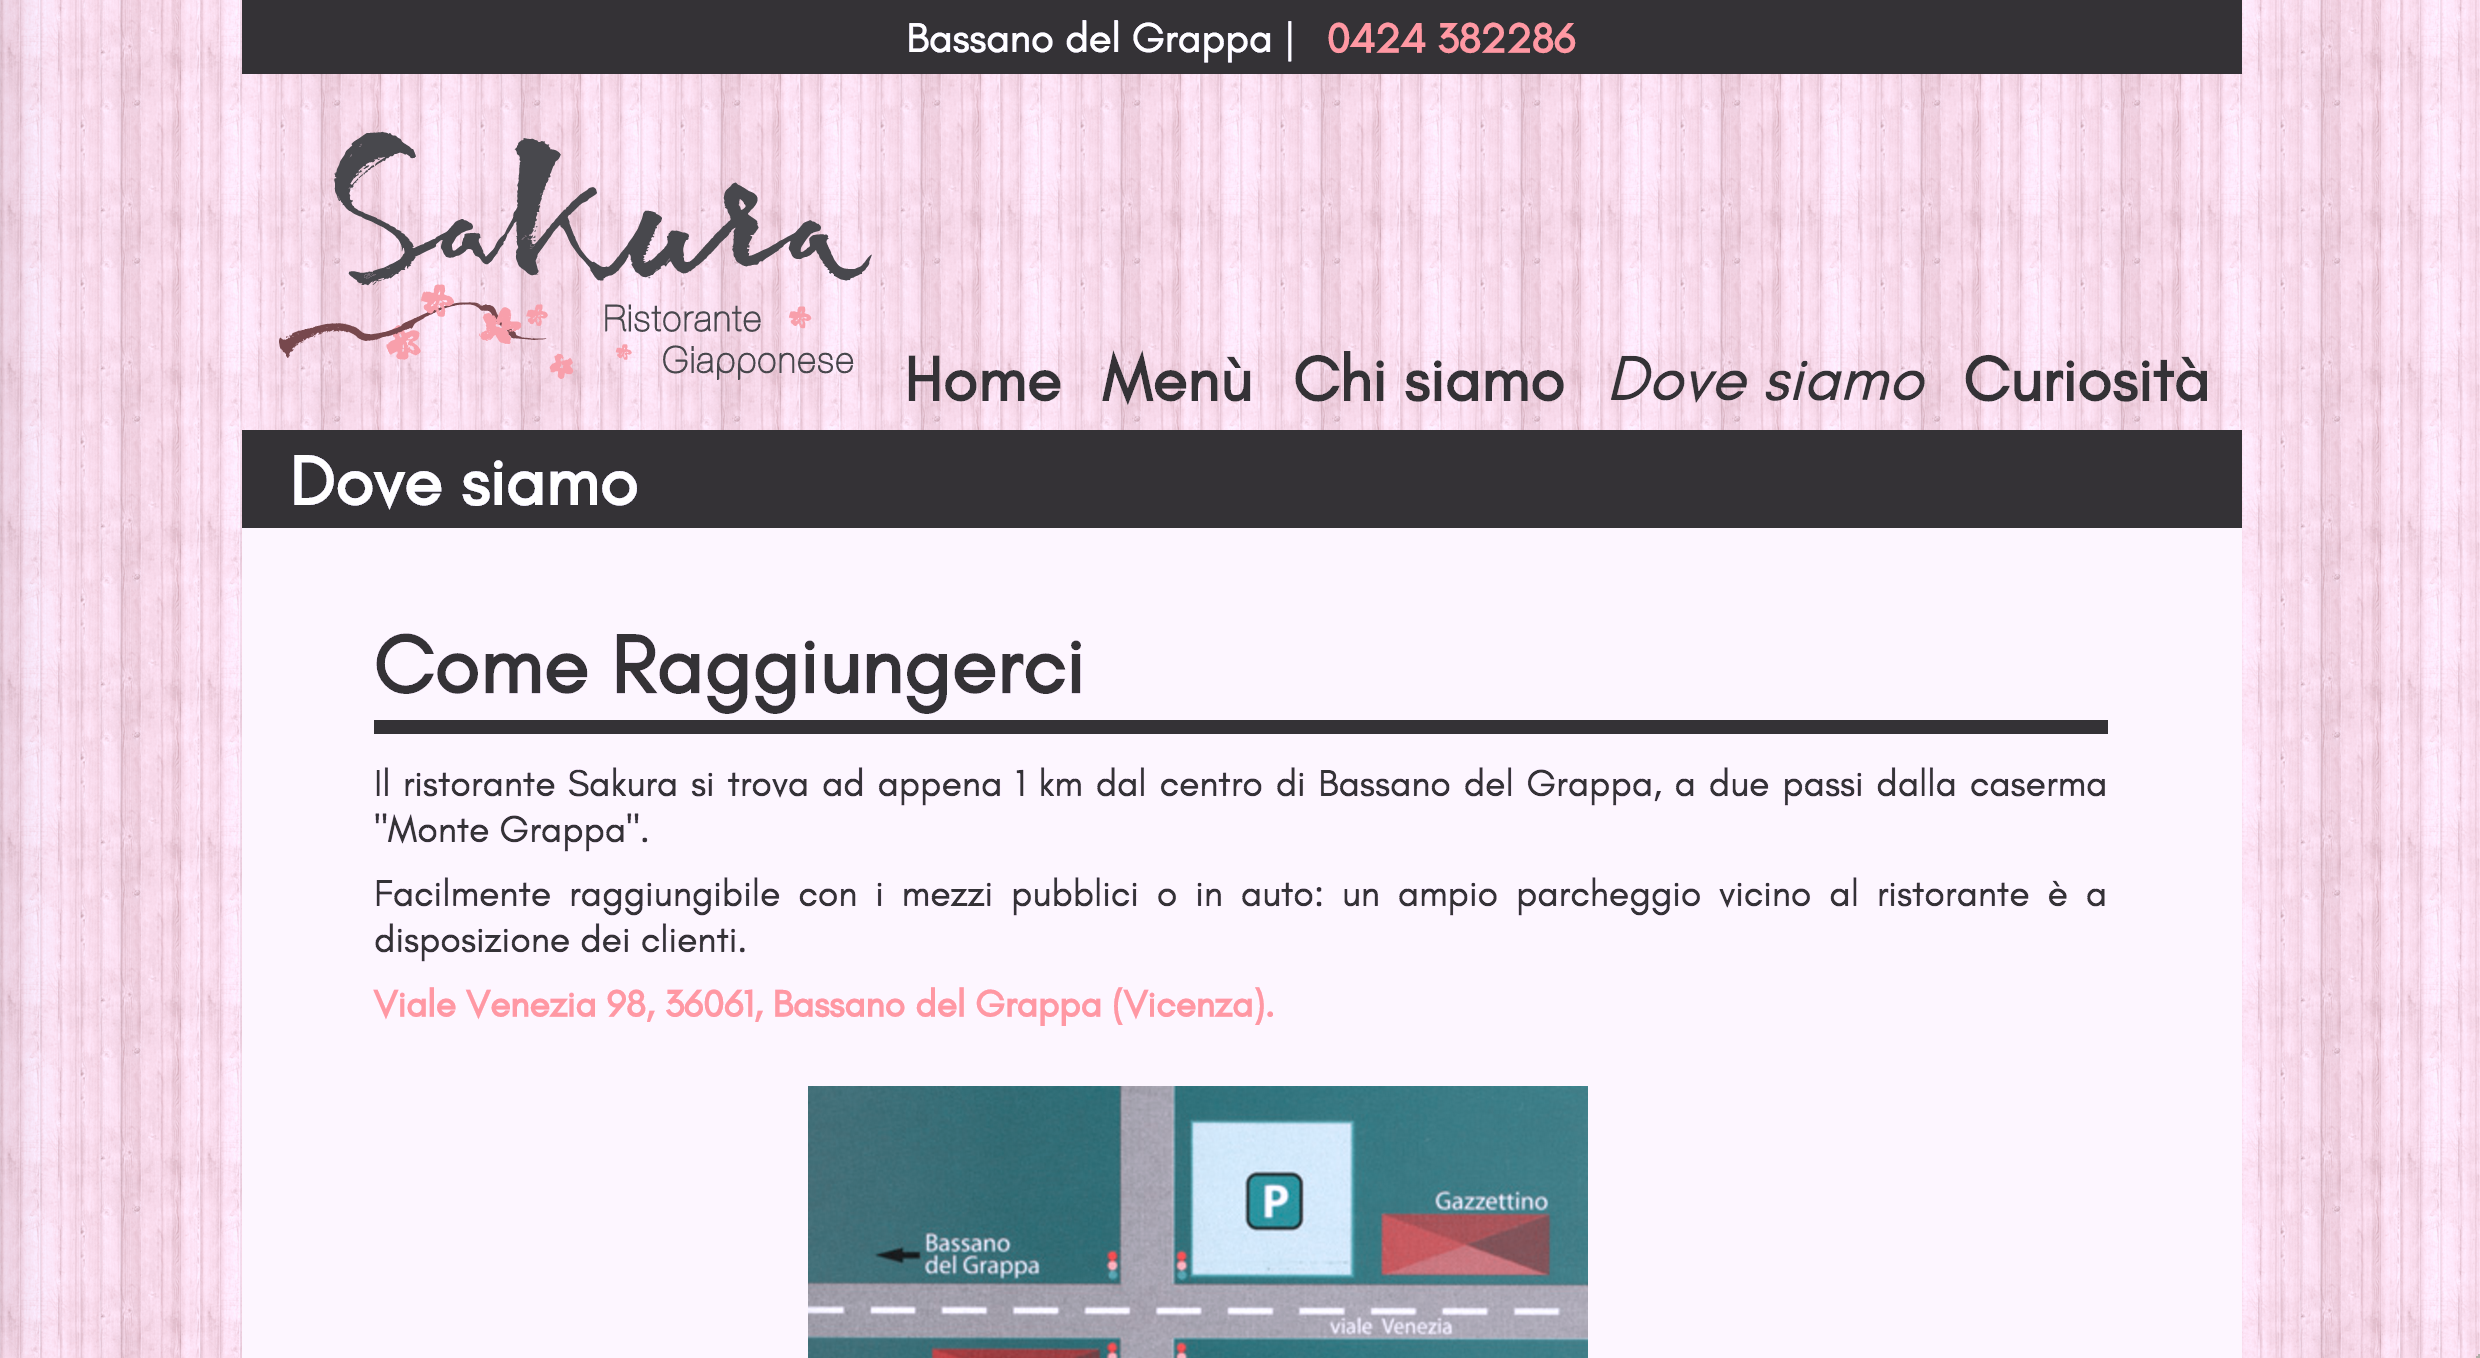
\includegraphics[width=\textwidth]{images/colorblindness/tritanopia}
		\caption{Esempio di pagina vista da chi soffre di tritanopia}
		\label{fig:Esempio di pagina vista da chi soffre di tritanopia}
	\end{figure}
	\begin{figure}[H]
	\centering
		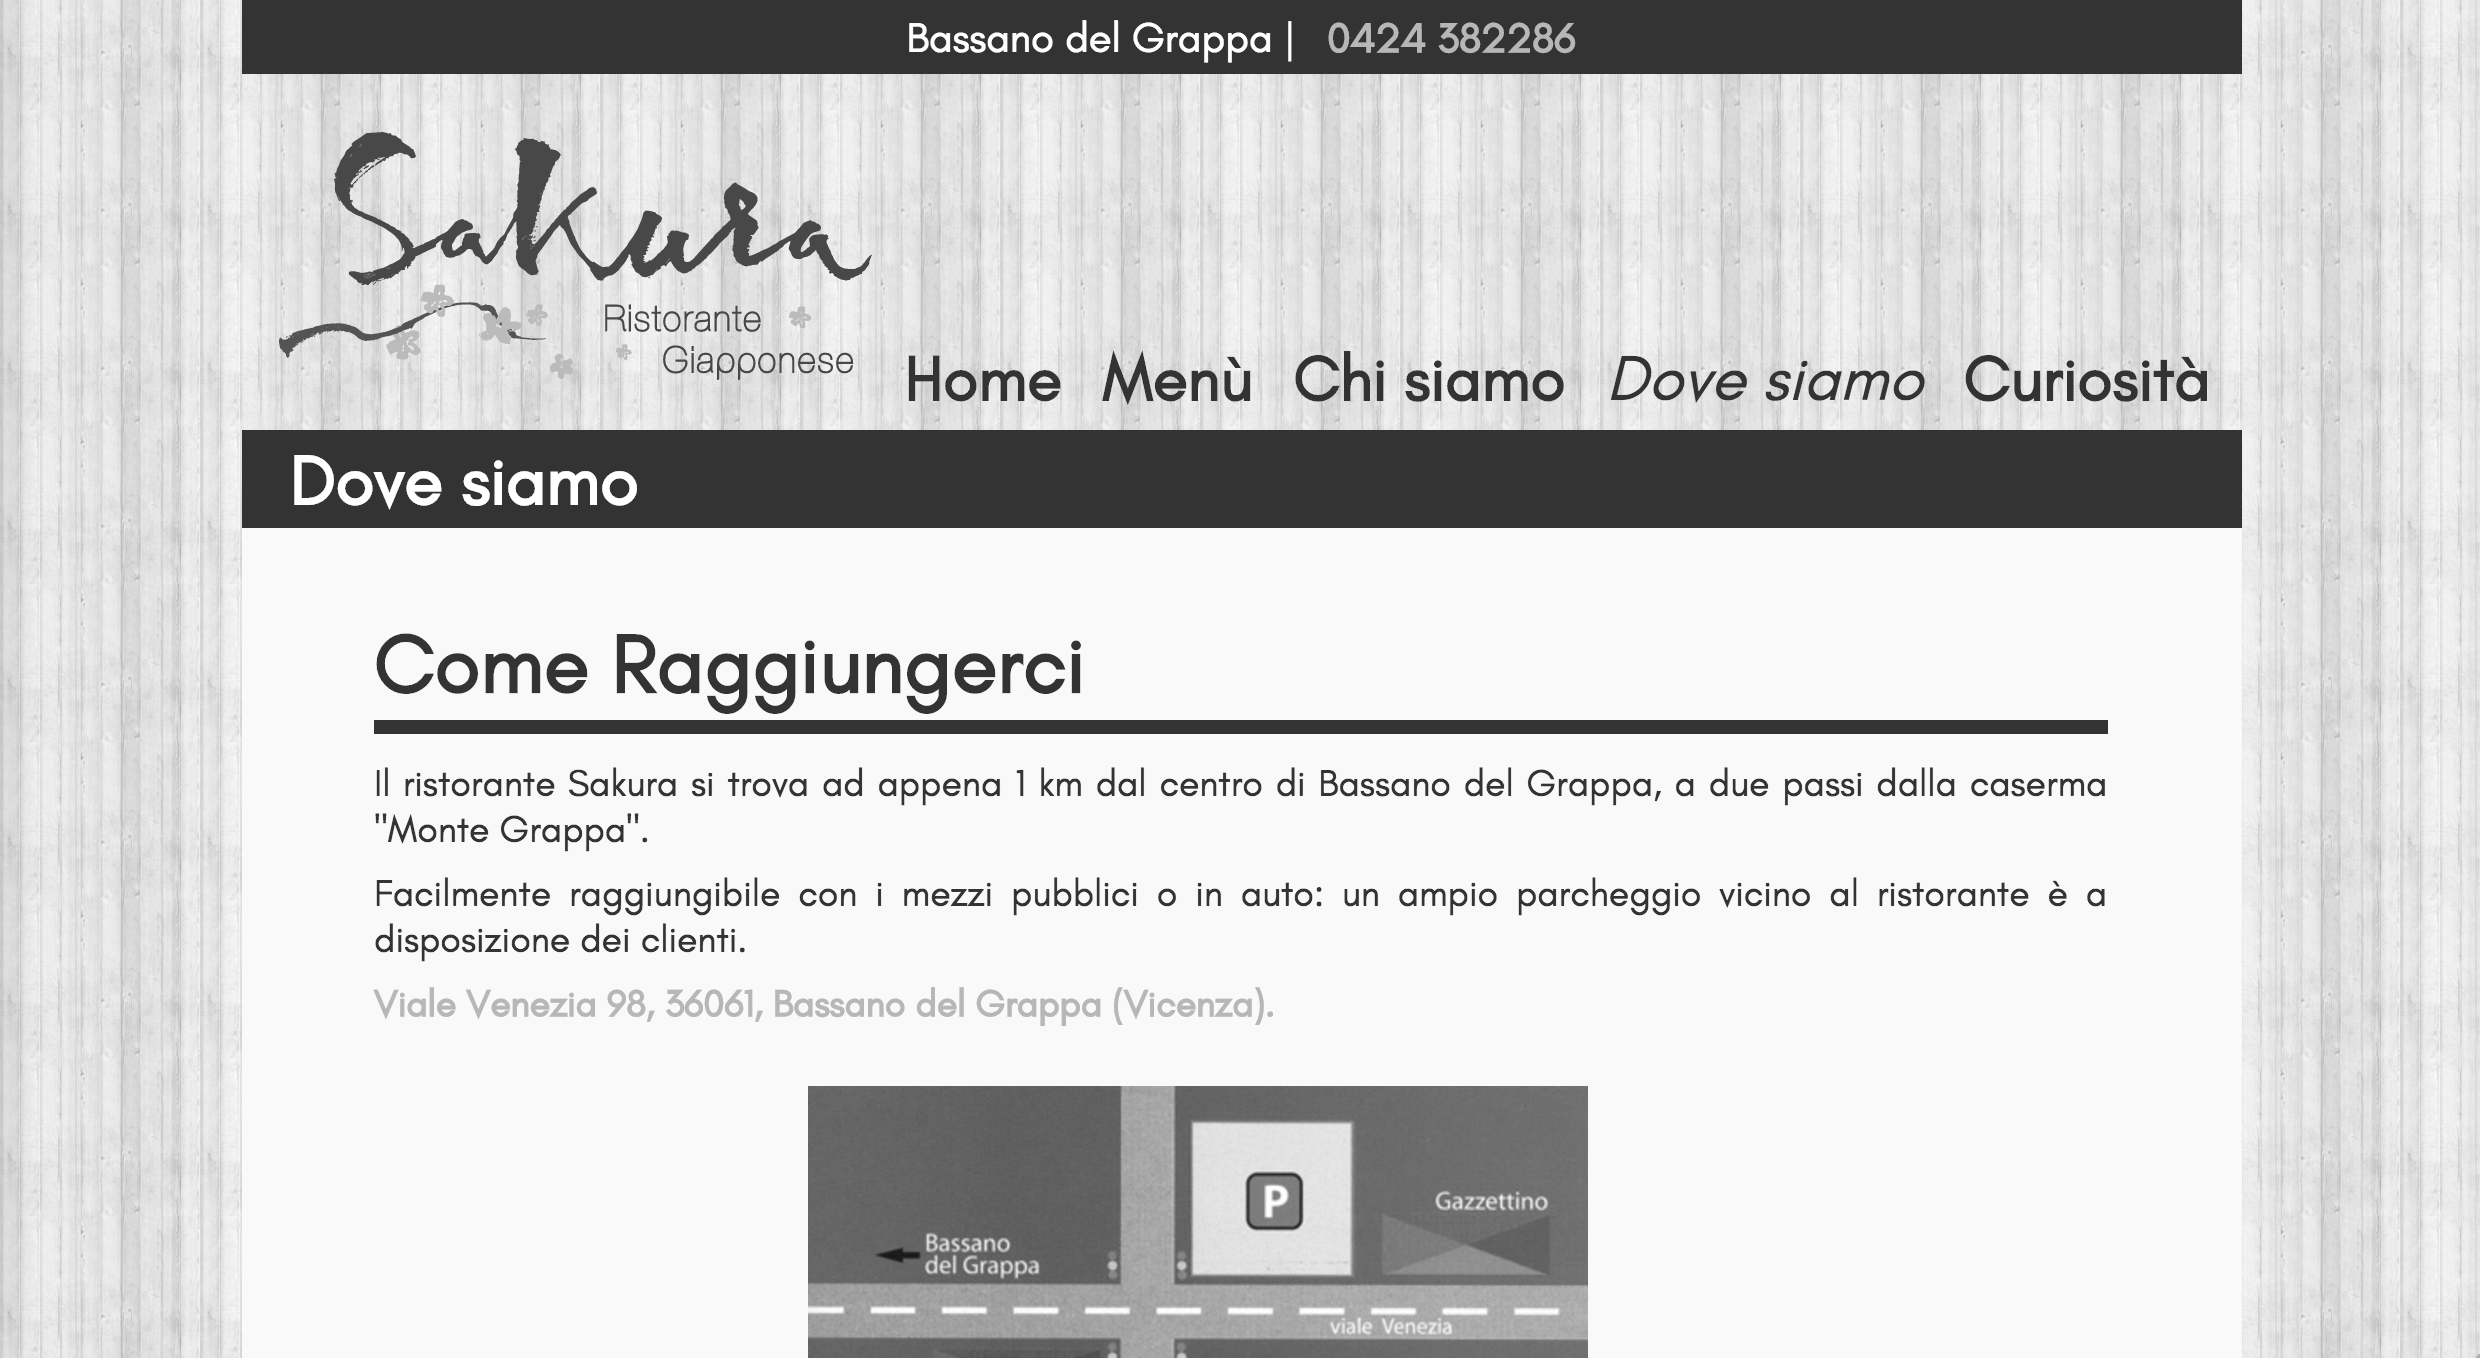
\includegraphics[width=\textwidth]{images/colorblindness/monochromacy}
		\caption{Esempio di pagina vista da chi soffre di monochromacy}
		\label{fig:Esempio di pagina vista da chi soffre di monochromacy}
	\end{figure}
	
	\subsection{Parole straniere}
		All'interno del sito sono presenti molte parole giapponesi, per ovvii motivi: in ognuno di questi casi è stato definito l'attributo \texttt{xml:lang="ja"} tra gli attributi del tag all'interno del quale figuravano (ad esempio, \texttt{strong}) oppure tra gli attributi di uno \texttt{span} opportunamente piazzato.\\\\
		All'interno del menù del ristorante invece sono presenti molte parole straniere: giapponesi, francesi, tedesche e spagnole: è stato definito uno \texttt{span} opportuno per ognuna di queste occorrenze, con attributo \texttt{xml:lang} impostato sulla lingua della parola straniera.\\\\
		Queste due operazioni hanno permesso di favorire la lettura del sito da parte di uno screen reader.
	
	\subsection{Form}
		Nella pagina \texttt{private-menu.cgi}, presente nell'area amministratore, è possibile effettuare delle modifiche al menù del ristorante.\\
		Nelle \texttt{form} di questa pagina si è preferito semplificare la parte di presentazione pur di mantenere la validazione dell’\texttt{XHTML} e quindi mantenere un buon livello di accessibilità.\\\\
		Si deve tenere conto anche del fatto che questa pagina è accessibile unicamente all'amministratore, quindi il sacrificio in fatto di presentazione è accettabile in quanto non si toglie nulla all'utente che visita il sito.\\\\
		Più in generale, in tutte le \texttt{form} del sito non è stata definita una \texttt{legend} perché il titolo della pagina, stampato con un \texttt{<h3>} proprio sopra la \texttt{form}, rende totalmente chiaro all'utente lo scopo della \texttt{form} ed il motivo per cui quei tag \texttt{input} sono raggruppati.\\\\
		Gli errori trovati durante l'inserimento di dati nelle form sono stati segnalati in maniera elegante, sfruttando il \texttt{Perl} per il controllo lato server ma anche il \texttt{Javascript} per un controllo immediato (se attivo) lato client.\\\\
		(\textbf{+ + + + + + + + aggiungere screenshot + + + + + + + +})
	
	\subsection{Accessibilità da tastiera}
		Una condizione necessaria ad un sito per essere accessibile è quella di essere navigabile utilizzando solamente la tastiera.\\
		Ogni pagina del sito è stata testata ed il risultato è che il sito è navigabile utilizzando \texttt{Tab} ed \texttt{Enter}, ad eccezione delle pagine \texttt{menu.cgi} e \texttt{private-menu.cgi} (rispettivamente, parte pubblica e amministratore) con \texttt{Javascript} attivo.\\
		Infatti, nel caso in cui \texttt{Javascript} non sia attivo, il sito è navigabile totalmente da tastiera.\\
		Il gruppo ha deciso di non utilizzare gli attributi \texttt{tabindex} per i \texttt{link} del sito in quanto il flusso logico del sito è semplice e lineare.
	
	\subsection{Accessibilità tramite screen reader}
		Riportare gli esiti dell'uso del sito con Lynx + \textbf{aggiungere screenshot}
		
\end{document}